\section{Experimental evaluation}
\label{sec:results}
\begin{figure*}[!Ht]
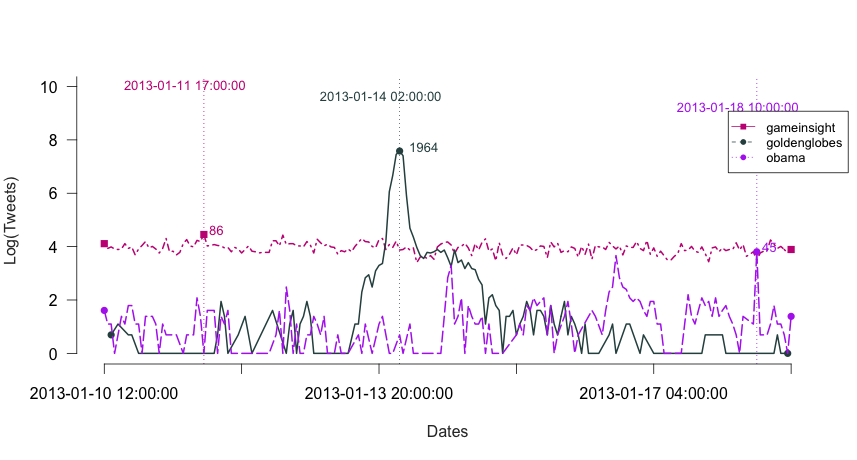
\includegraphics[width=0.9\textwidth]{images/3-plots.png} 
\caption{Popularity over time of three hashtags: gameinsight, goldenglobes and obama. Number of tweets have been normalized through the \emph{log} function}
\label{fig:trends}
\end{figure*}

\begin{figure*}[!Ht]
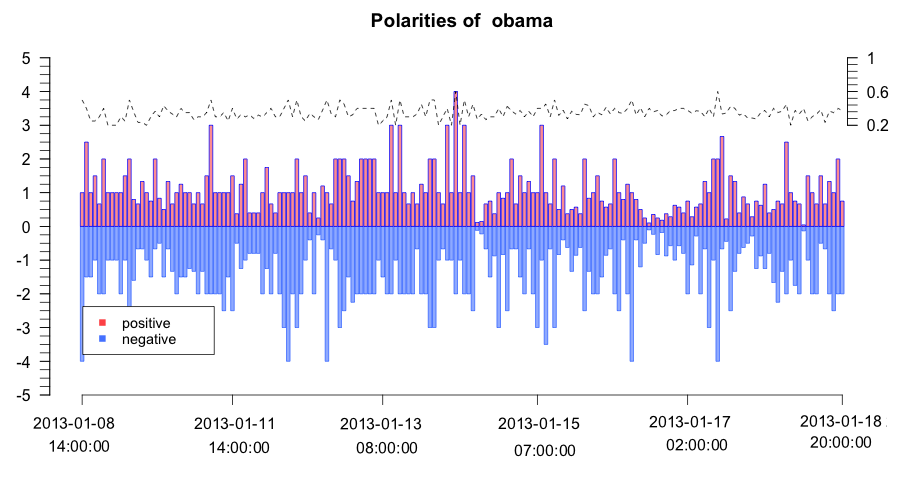
\includegraphics[width=0.9\textwidth]{images/obama-sentiment.png} 
\caption{Sentiment polarity expressed through tweets containing the hashtag ``obama''. The dashed line on the top, represent in each point in time the average emotional divergence.}
\label{fig:obama-sentiment}
\end{figure*}

\begin{figure*}[!Ht]
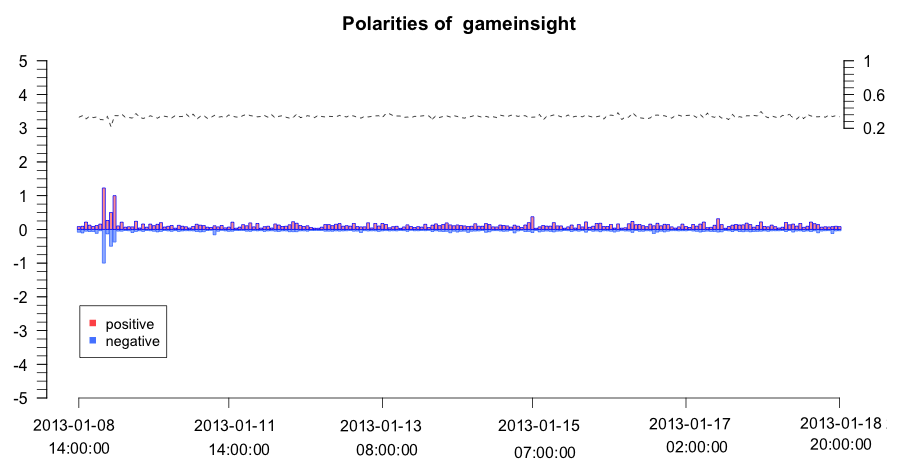
\includegraphics[width=0.9\textwidth]{images/game-sentiment.png} 
\caption{Sentiment polarity expressed through tweets containing the hashtag ``gameinsight''. The dashed line on the top, represent in each point in time the average emotional divergence.}
\label{fig:game-sentiment}
\end{figure*}



We tested our solution with Stratosphere 0.2.1\footnote{\url{https://stratosphere.eu/downloads}} running on a GNU/Linux machine with 2Gb RAM DDR2, and a CPU AMD Athlon\texttrademark 64bit X2 Dual Core Processor 5000+.%\footnote{Linux 3.0.0-12-generic \#20-Ubuntu SMP x86\_64}. 
We used a version of Stratosphere which is not publicly available at the time of writing as still in beta-testing.
%Bugs present in the current implementation limited the degree of parallelism to 1.

All the experiments have been performed on samples of the original database, in order to show time and quality performance. 
We used Java JRE 1.6.0\_26 to program the PACT using the Stratosphere libraries and server, additionally we integrated the SentiStrength java library\footnote{\url{http://sentistrength.wlv.ac.uk}}. 
We performed preliminary experiments to set the english word threshold and we finally set it to $\sigma=0.1$, i.e., requiring at least 1 word out of ten being a valid English word.
%, in order not to prune too many tweets. 
Since we are matching with english words that are not stemmed a larger threshold would have pruned interesting tweets.  

\subsection{Time performance}
%Describe the time over the (number of threads [if we could]? size of the database)
In this section we briefly report and comment time performance registered in the various experiments.
We performed a total of 4 different experiments testing the flow on different dataset sizes. 
%, where the flow and so the statistics retrieved where always the same, but we changed the set of tweet over which we computed them.

%As said before we performed this experiment with a degree of parallelism se to 1.
%This means that Stratosphere had been instructed to compute each step sequentially without exploiting possible parallel computations.
In particular we run over the last 100 thousands, 1 million, 10 million and 20 million tweets, in reverse chronological order.
Time results are present in table~\ref{tbl:times}. 

As expected, we registered time performance rapidly increasing with respect to the number of tweets.
Although the dataset is big and the computed statistics are complex we measured a total time of at most 1 hour for 20 millions tweets in the worst case.

\begin{table}[htb]
\centering 
\begin{tabular}{|l|r|}
\hline		
Number of Tweets			& Time (secs)\\
\hline
$100$ thousands tweets		&	50\\
$1$ million tweets		& 183\\
$10$ million tweets 		& 1516\\
$20$ million tweets 		& 4006\\  
\hline
\end{tabular}
\caption{Time performances for the computation of the statistics with respect to the size of the dataset analyzed}
\label{tbl:times}
\end{table}

\begin{figure}[!ht]
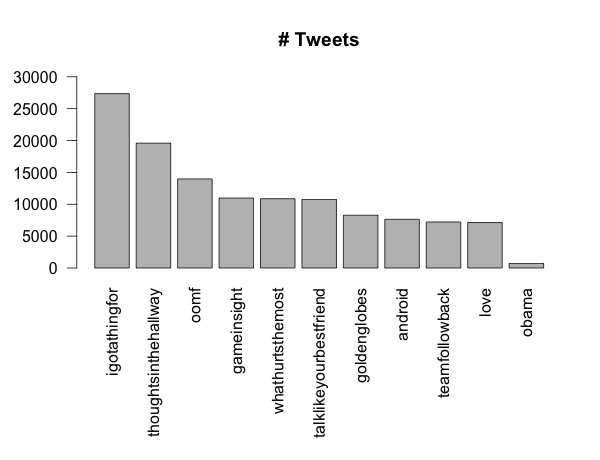
\includegraphics[width=0.45\textwidth]{images/hashtag-tweets-hist_20.png} 
\caption{Top10 hashtags for popularities within tweets, plus the hashtag for ``obama'' vs the number of tweets in which they appear}
\label{fig:tweets-hist}
\end{figure}

\begin{figure}[!hb]
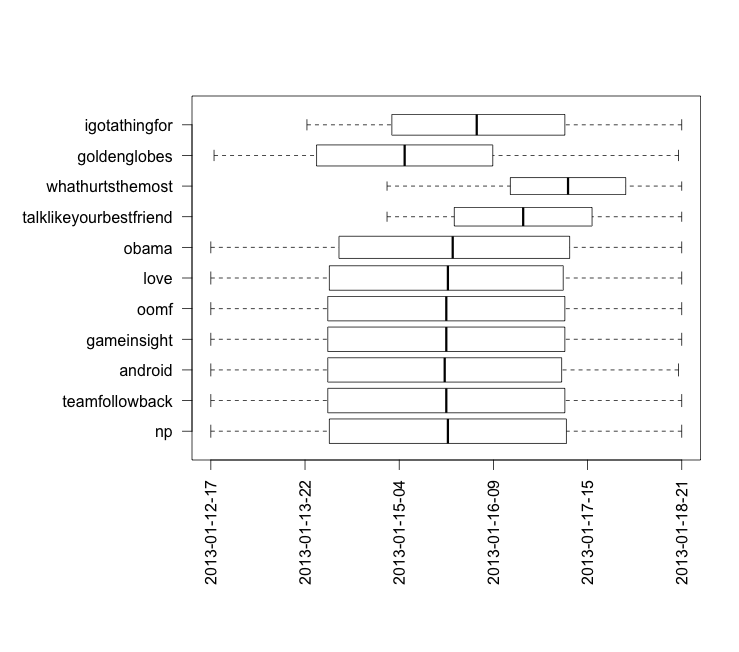
\includegraphics[width=0.45\textwidth]{images/hashtags-timewindow.png} 
\caption{Lifespan of the Top10 hashtags plus ``obama'' the thicker line delimits where the first and third quartile of tweets for that hashtag lies}
\label{fig:tweets-lifespan}
\end{figure}

\subsection{Output charts}
% describe how we used the data and which parameters we extract. 
%As described previously, the scope of this work is building a flow that can cope with a large amount of tweets, and which can parse, clean and filter them.
%Moreover this flow is designed to compute and aggregate statistics for the hashtags present in the flow and can be extended  to many more analysis.
Starting from our initial assumption, i.e., hashtags  are indicators of events or discussion topics, we experimentally show how our PACT flow can find important patterns in our data.

\begin{table}[htb]
\centering 
\begin{tabular}{|l|r|}
\hline		
Hashtag			& Number of Tweets\\
\hline
obama		&	1771\\
obamacare		& 173\\
nobama 		& 120\\
impeachobama 		& 73\\  
obama2012 		& 63\\  
\hline
\end{tabular}
\caption{Hashtags referring to ``Barack Obama'' and the number of tweets containing them}
\label{tbl:obama-tweets}
\end{table}

In Figure~\ref{fig:tweets-hist} we show the Top10 hashtags for popularity, plus the hashtag for ``obama'' as a possibly interesting case  and we analyze their lifespan in Figure~\ref{fig:tweets-lifespan}.
Indeed, identifying that an hashtag has a limited lifespan within the flow of tweets may provide anecdotal evidence of an event happening in that  particular time window.
Looking instead to the hourly evolution of the popularity of each tweet we can identify interesting trends, points of peeks and lows.
In Figure~\ref{fig:trends} we can see how the popularity of some hashtags (expressed as hourly number of tweets), can have very different evolutions.
In that figure the hashtag ``gameinsight'' refers to the name of one developer and publisher of mobile games and social games, they and their followers use this hashtag when referring to some of these games.
We can see that during the time of the analysis the number of tweets mentioning this tag each our is pretty stable.
Instead, the other two hashtags have some highly unstable behavior.
The one referring to Barack Obama is not so much popular, even considering all the possible hashtags talking about president Obama, as we shown in Figure~\ref{tbl:obama-tweets}.
In contrast to the previous hashtag, the hourly number of tweets containing the tag ``obama'' is more unstable, and we can see that there are time windows where this number is actually zero.
Finally, in Figure~\ref{fig:trends} , we analyze also tweets regarding the ``goldenglobe'' hashtag, referring to the annual Golden Globe Awards, held in 2013 on the night of 13Th. of January.
The data-peak we can observe is an indicator of when the award night where held exhibiting a burst in the trend.
%, and we can easily see how before and after that peek was and returned to be pretty low.

Finally, another information to take into account, about the evolution of an event, is the polarity expressed in tweets about it.
In Figure \ref{fig:obama-sentiment} and ~\ref{fig:game-sentiment} we show average emotional polarities present in tweets in the hourly time-window.
These pictures demonstrates how while tweets containing the ``gameinsight'' keyword are more popular, tweets tagged with the hashtag ``obama'' have a more strong weight in terms of sentiment polarities.
These statistics combined with the evolution of popularity of hashtags are starting points for more complex models and analysis.
They can be used to actually identify which hashtags in which time windows are likely to be indicator of events happening.
Furthermore, approaches like the ones presented in \cite{Vlachos:2004:ISP:1007568.1007586} can be applied not only to identify burst in popularity or in sentiment polarities, but also to identify overlapping bursts, i.e. bursts in popularity for different hashtags in the same time window, so that we can actually detected which hashtags may refer to the same event.

In the end of our process we are able to aggregate, for the biggest dataset at our disposal, statistics for  more than 480 thousands hashtags, keeping tweets from more than 604 thousands users over 247 time windows.
These aggregated statistics can easily be used as grounds for more complex and structured reasoning, but they are already able to highlight popular hashtags.




